\documentclass[12pt]{article}
\usepackage{hyperref}
\usepackage[warn]{mathtext}
\usepackage[T2A]{fontenc}
\usepackage[utf8]{inputenc}
\usepackage[russian]{babel}
\usepackage{cite}
\usepackage{amsfonts}
\usepackage{lineno}
\usepackage{subfig}
\usepackage{graphicx}
\usepackage{xcolor}
\usepackage{bm}
\usepackage{graphicx}
\usepackage{amssymb}
\usepackage{hyperref}
\usepackage[left=2cm,right=2cm,top=2cm,bottom=2cm]{geometry}
\usepackage{indentfirst}
\DeclareSymbolFont{T2Aletters}{T2A}{cmr}{m}{it}

\DeclareGraphicsExtensions{.png,.jpg,.svg,.pdf}
\author{Карцев Вадим}
\date{7 октября 2021 г.}
\title{Лабораторная работа 5.6

Измерение $\beta$-спектров с помощью сцинтилляционного пластикового детектора}

\begin{document}

  \maketitle

  \textbf{Цель работы:} Определение граничных энергий распада различных элементов.

  \textbf{В работе используются:} Сцинтилляционный пластиковый детектор частиц,
  персональный компъютер, кюветы с источниками излучения $^{137}Cs$, $^{90}Sr$,
  $^{36}Cl$, $^{60}Co$, $^{22}Na$, монета.

  \section{Аннотация}

    В данной работе мы изучили спектры $\beta$-излучения Cs, Sr, Cl, Na и Co.
    Также мы изучили спектры $\gamma$-излучения возбужденных атомов, полученных
    в ходе $\beta$-распада этих элементов. По этим спектрам мы оценили граничные
    энергии $\beta$-распада и энергии комптоновского края.

  \newpage
  \section{Теоретическая справка}

    В сцинтилляционном пластиковом детекторе световые вспышки возникают за счет
    взаимодействия электронов с материалом детектора. Электроны могут попадать
    туда от внешнего $\beta$-активного источника, либо появляться
    непосредственно в материале детектора за счет взаимодействия
    $\gamma$-квантов от внешнего источника излучений. Такими процессами является
    фтоэффект, комптоновское рассеяние и рождение электрон-позитронных пар.

    В большинстве случаевы искусственные источники гамма-излучения являются
    бета-источниками, в которых после бета-распада образуется дочернее ядро в
    возбужденном состоянии. В данном случае имеем дело с бета-переходом из
    $^{60} Co$ в ядро $^{60} Ni$.

    \begin{figure}[h!]
      \begin{minipage}[h]{\linewidth}
        \center{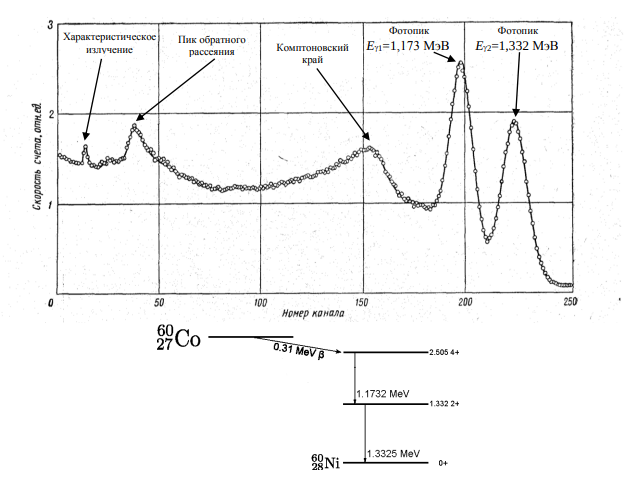
\includegraphics[width=0.75\linewidth]{theory.png}}\\
        Рис 1. Гамма-спектр радиоактивного источника $^{60} Co$, полученный при
        регистрации излучения сцинтилляционным гамма-спектрометром с кристаллом
        $NaI(Tl)$. В нижней части рисунка показана схема распада этого ядра.
      \end{minipage}
      \label{chart:theory}
    \end{figure}

    Время жизни этого гамма-источника определяется периодом полураспада
    $^{60}Co$, равного $5,2$ года, а время гамма-переходов при снятии
    возбуждения в ядре $^{60}Ni$ очень мало $(\approx 10^{-10} c)$\\


  \newpage
  \section{Обработка данных для $^{137}Cs$}

    \begin{figure}[h!]
      \begin{minipage}[h]{\linewidth}
        \center{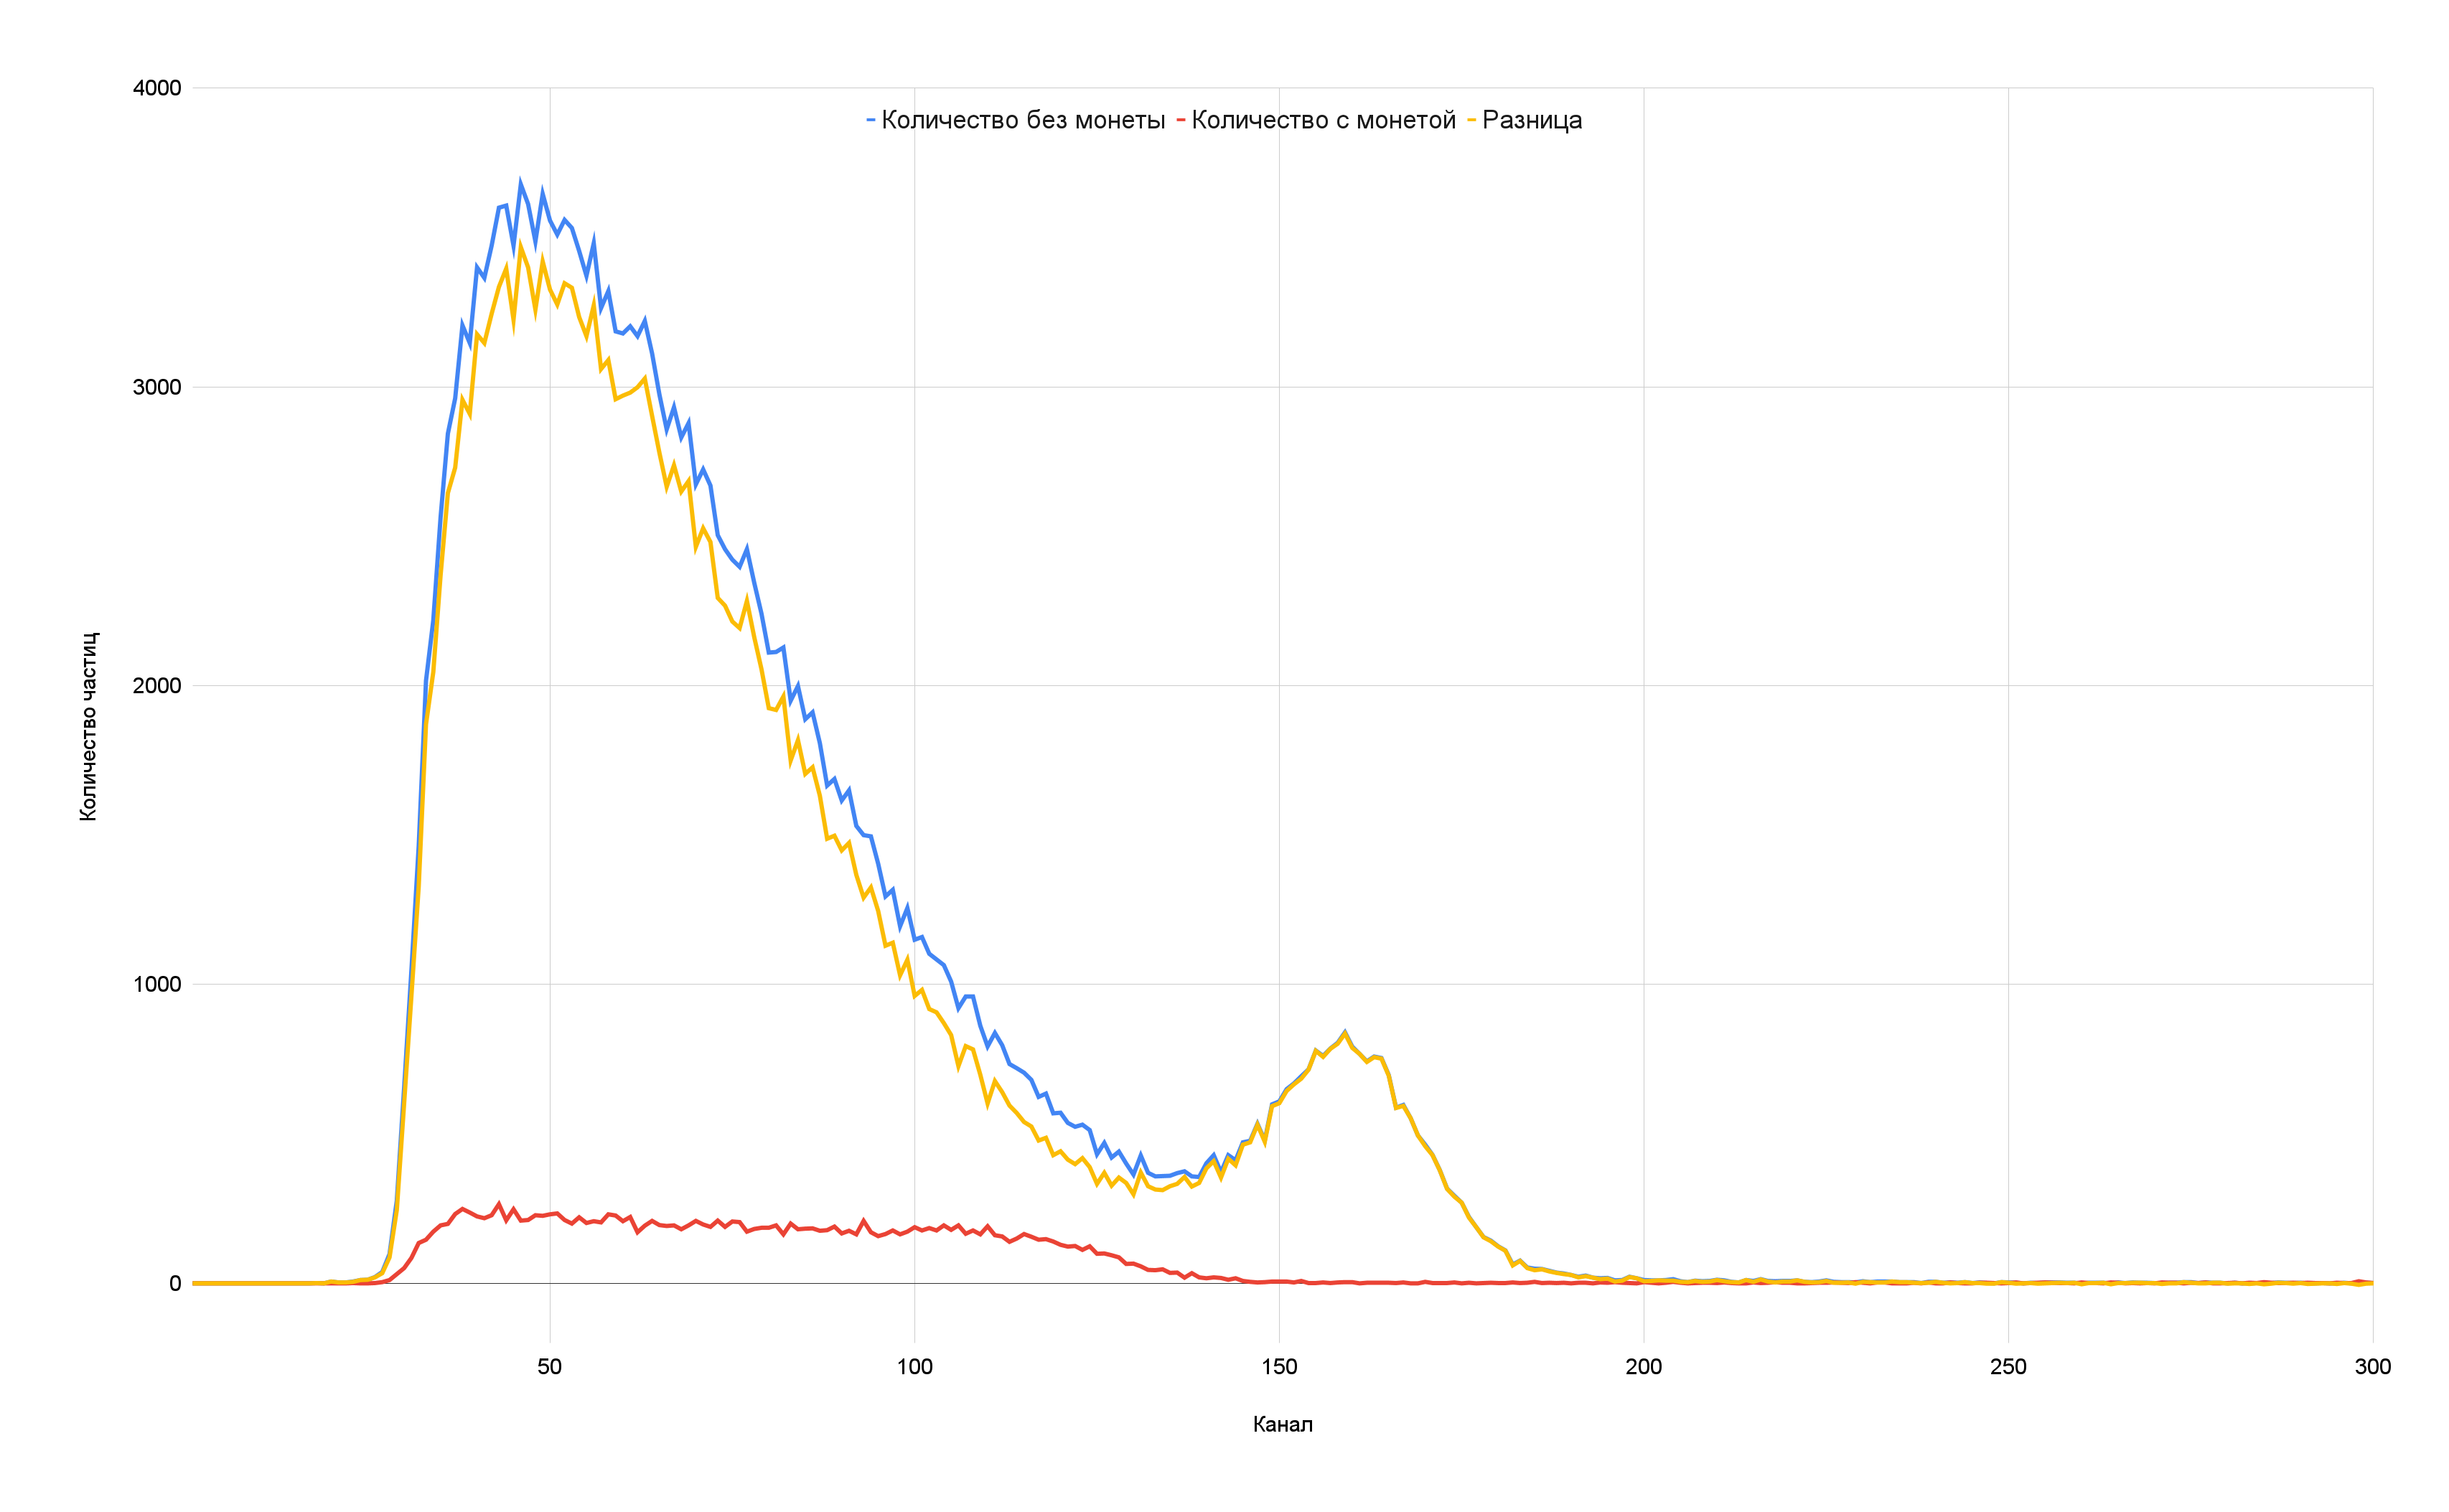
\includegraphics[width=\linewidth]{cesium.png}}
        Рис 3. Спектры для цезия без монеты и с монетой, разница спектров
      \end{minipage}
      \label{chart:cesium}
    \end{figure}

    \begin{figure}[h!]
      \begin{minipage}[h]{0.55\linewidth}
        \center{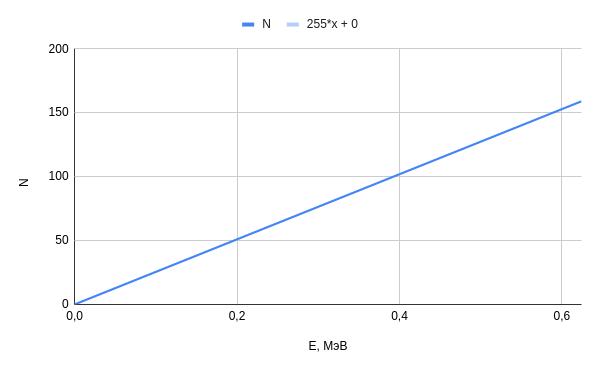
\includegraphics[width=\linewidth]{calibrating_plot.png}} \\
        Рис 4. Калибровочный график
      \end{minipage}
      \begin{minipage}[h]{0.44\linewidth}
        Виден пик, соответствующий конверсионным электронам с энергией
        $E_k = 0.624$ МэВ. Номер канала этого пика $N_k = 159$.
        Зависимость $N_i = \alpha E_i \Rightarrow$ построим калибровочный
        график.

        Тогда зависимость номера канала от энергии электрона:
        $N_i = 255 \cdot E_i$.

        Используя калибровочный график и спектр цезияс монетой получаем энергию
        края комптоновского рассеяния $E_k = 110/255 \approx 0,431$МэВ.

        Из $\beta$-спектра определим граничную энергию электронов:
        $E = 130/255 \approx 0,510$МэВ.

        Полученные данные совпадают с теоретическими значениями.
      \end{minipage}
      \label{chart:calibr}
    \end{figure}


  \newpage
  \section{Обработка данных для $^{90}Sr$}

    \begin{figure}[h!]
      \begin{minipage}[h]{\linewidth}
        \center{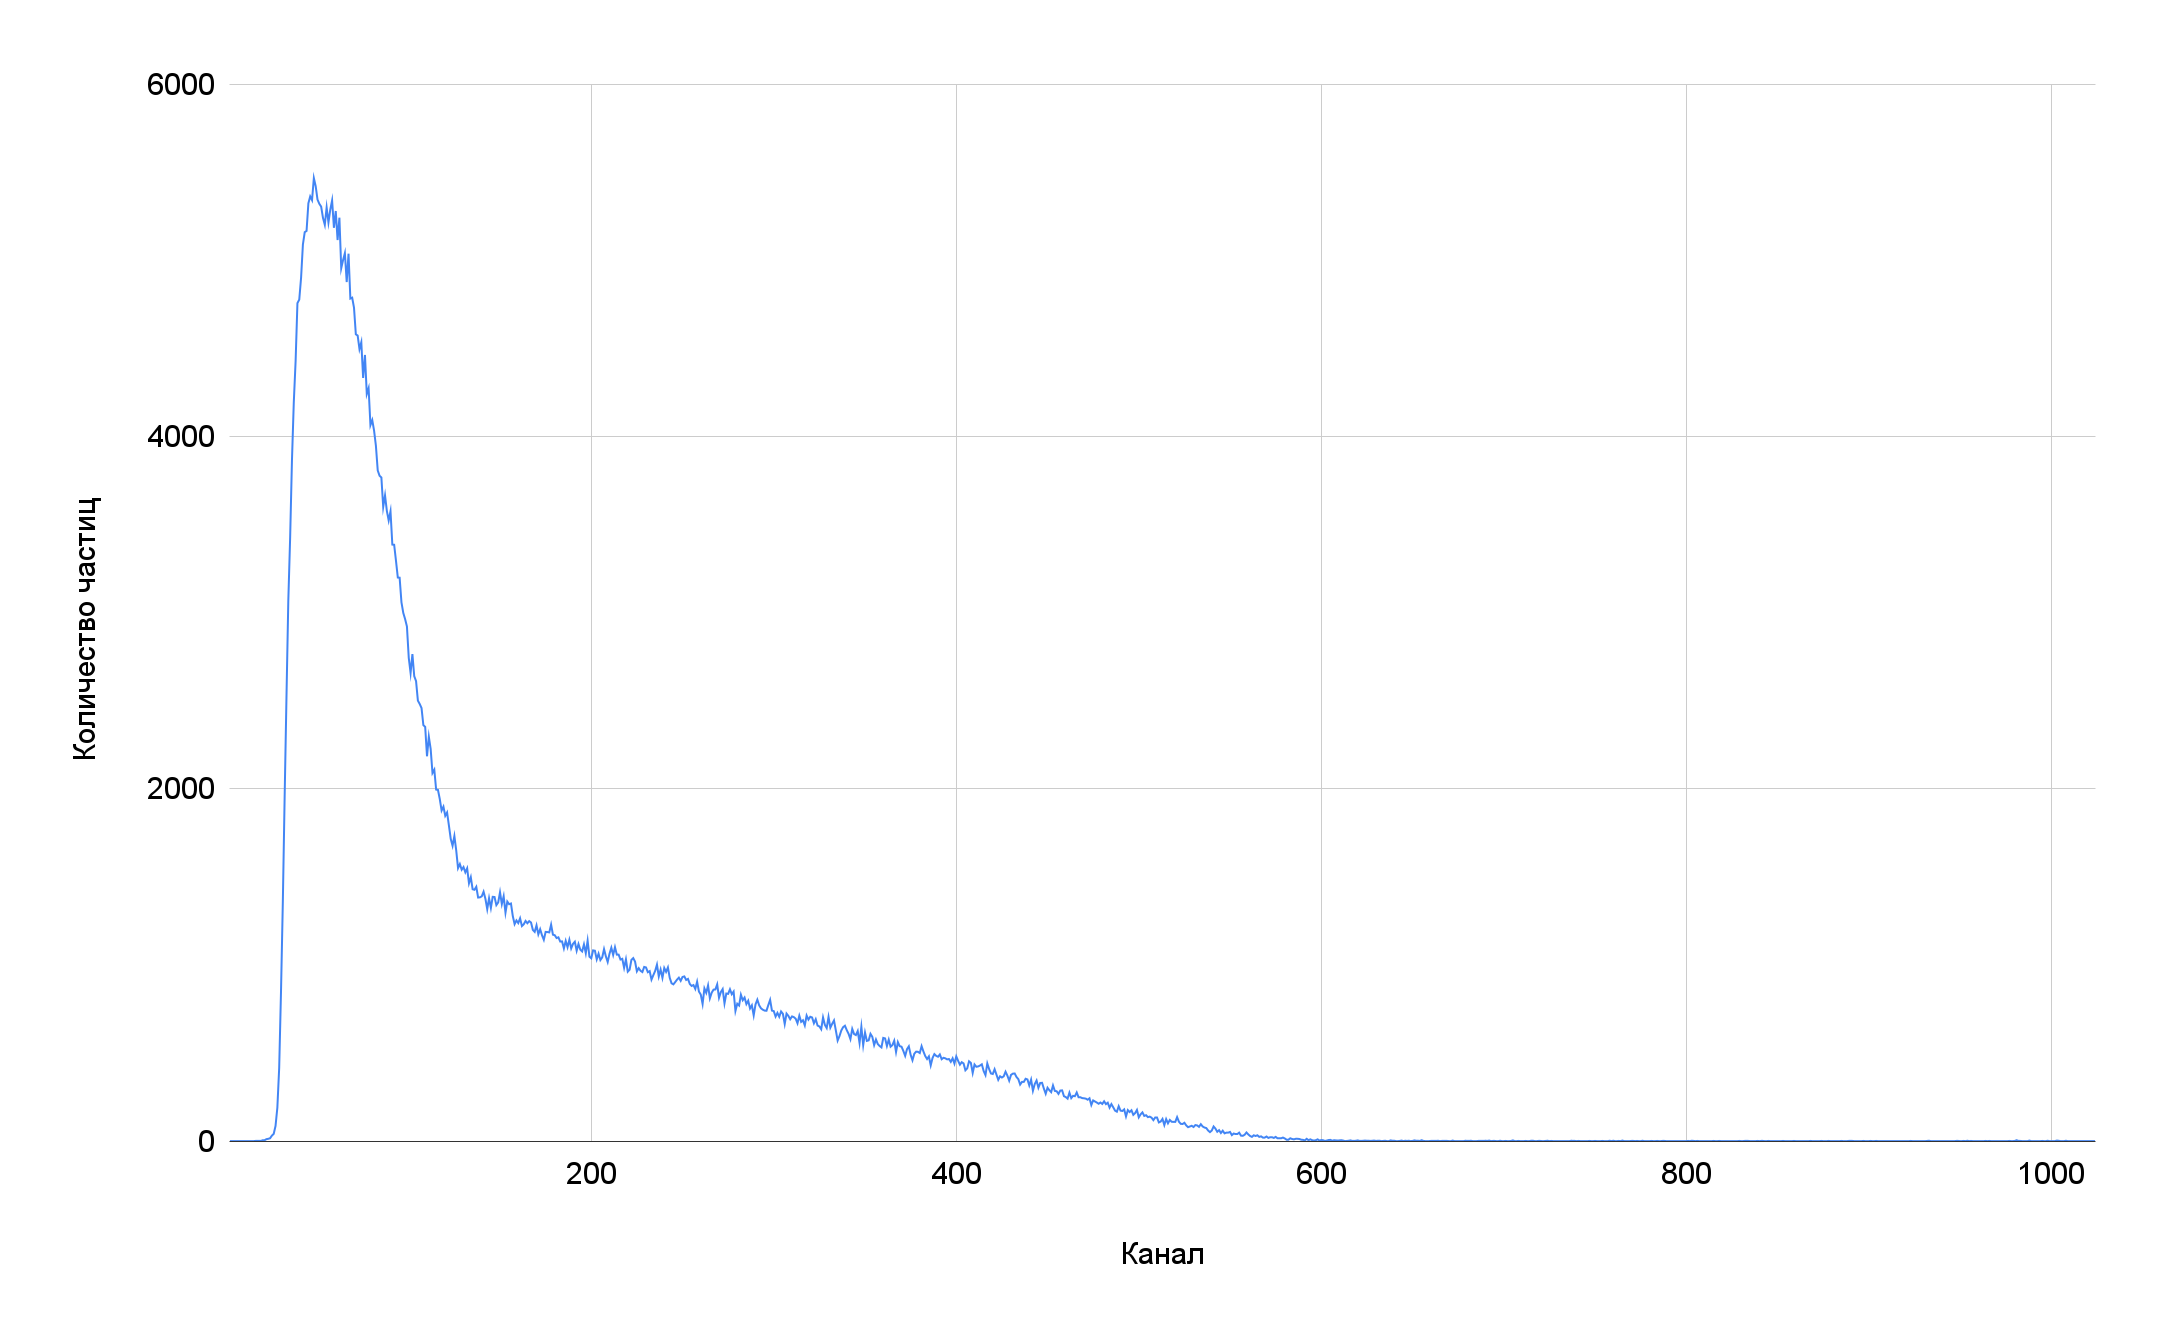
\includegraphics[width=\linewidth]{strontium.png}}
        Рис 2. Спектр для стронция
      \end{minipage}
      \label{chart:strontium}
    \end{figure}

    Из графика определим граничные значения электронов:$E_{Sr} = 145/255
    \approx 0.569$МэВ; $E_Y = 564/255 \approx 2.212$МэВ.

    Теретические значения: $E_{Sr} = 0.546$МэВ; $E_Y = 2.273$МэВ.


  \newpage
  \section{Обработка данных для $^{36}Cl$}

    \begin{figure}[h!]
      \begin{minipage}[h]{\linewidth}
        \center{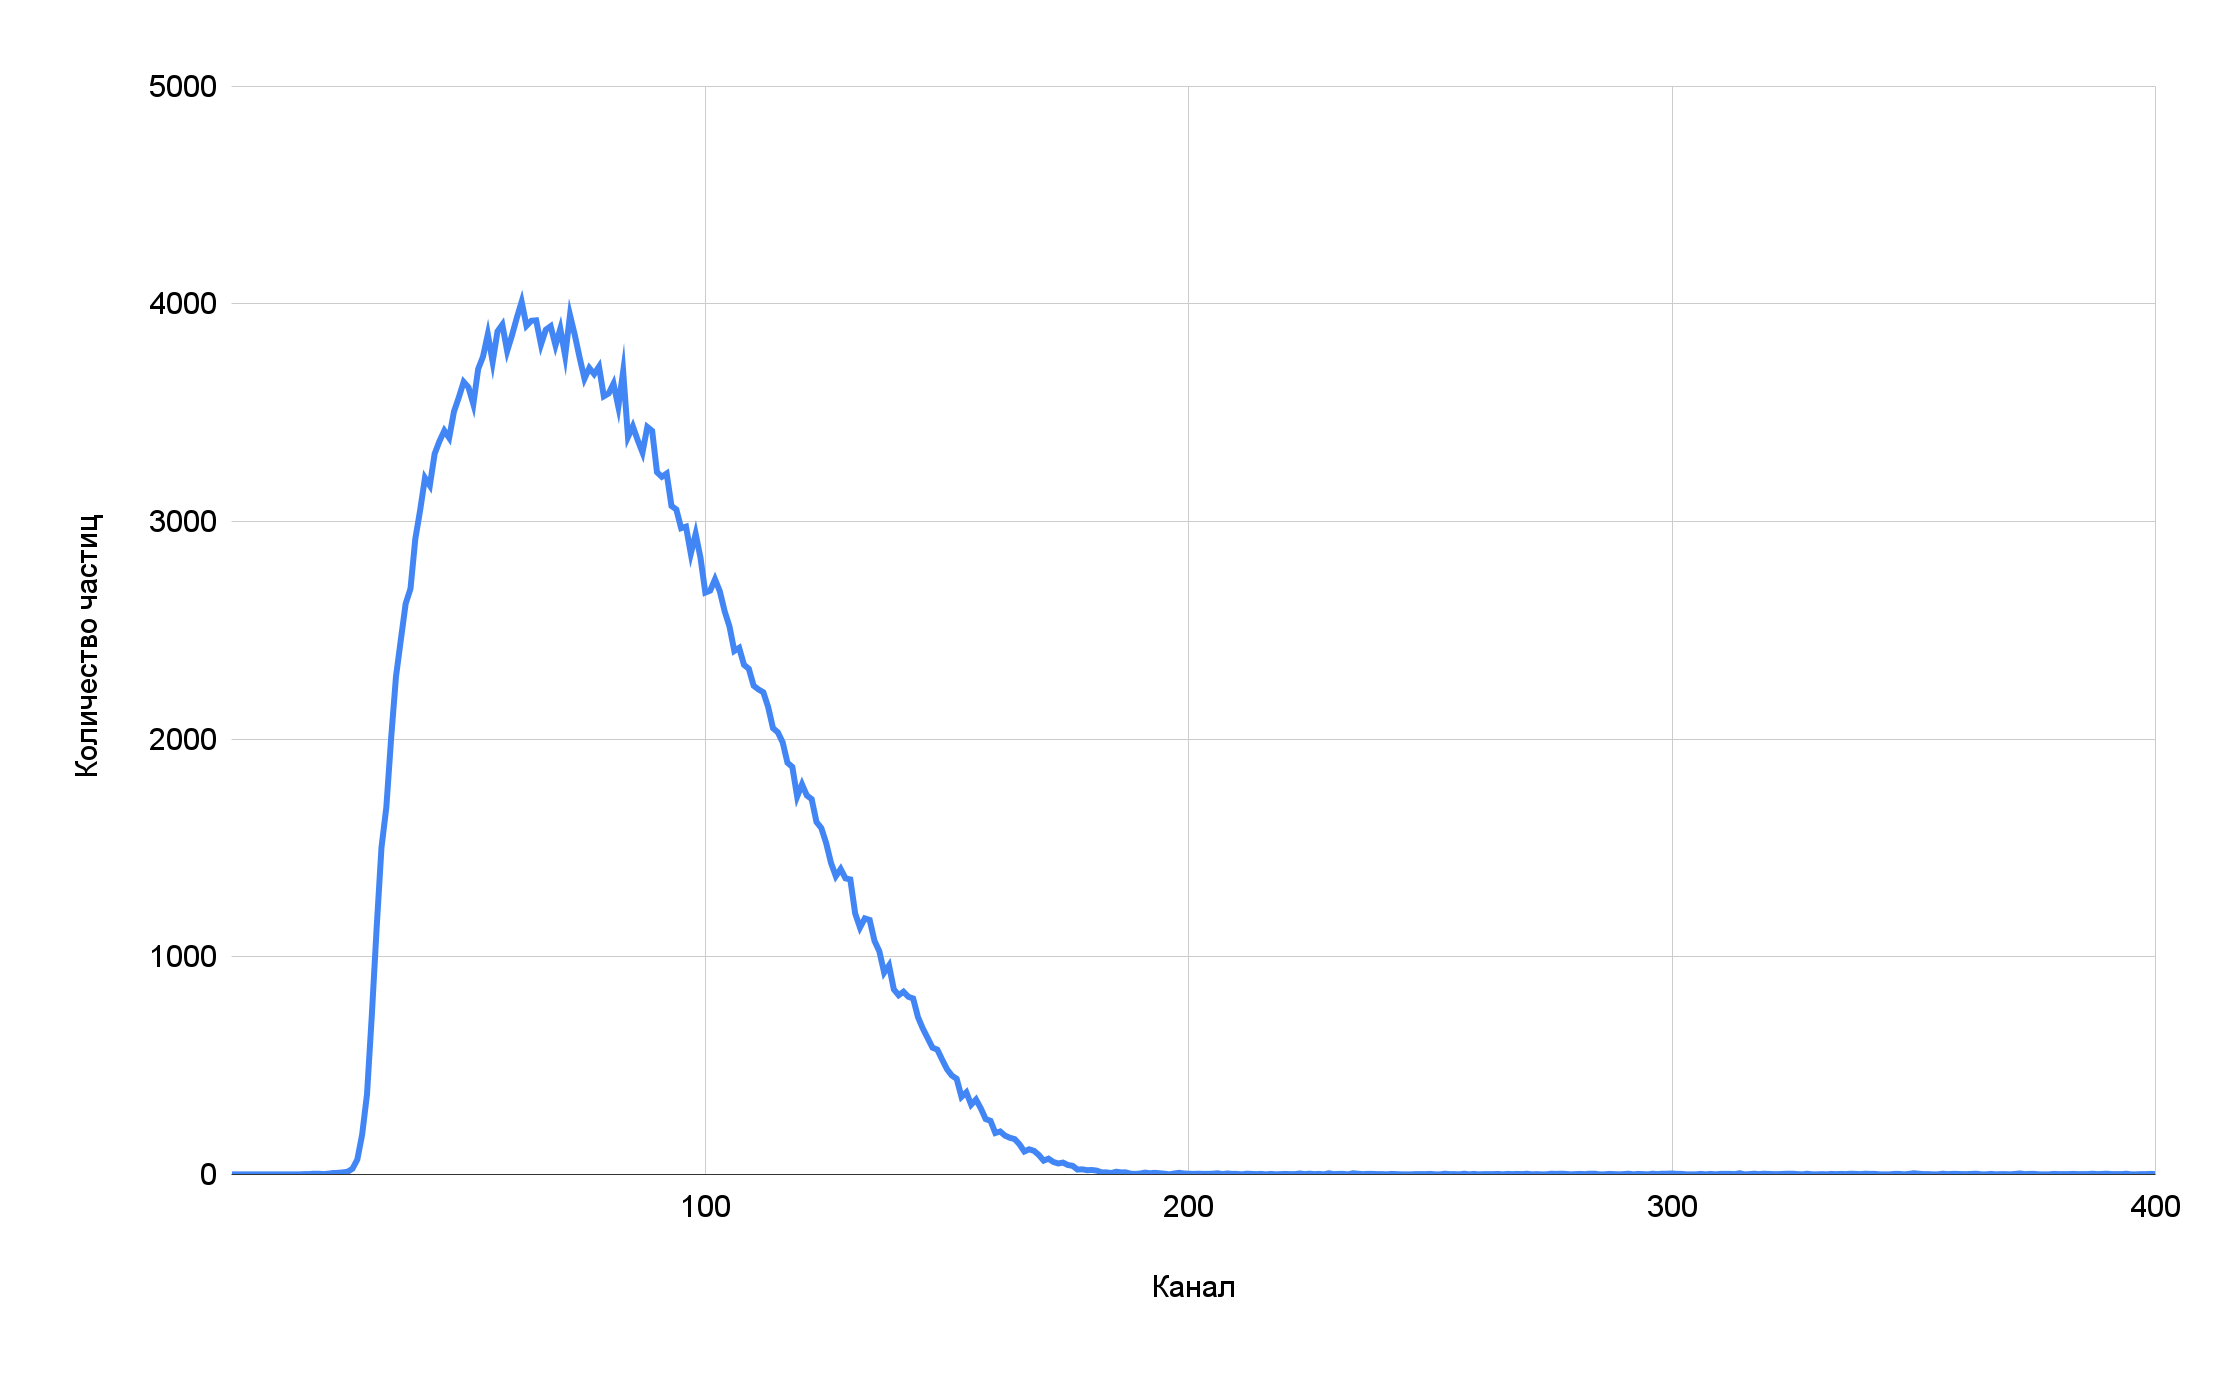
\includegraphics[width=\linewidth]{chlorine.png}}
        Рис 3. Спектр для хлора
      \end{minipage}
      \label{chart:chlorine}
    \end{figure}

    Граничная энергия электронов при и $\beta$-распаде: $E = 178/255
    \approx 0.698$МэВ.

    Теоретическое значение: $E = 0.714$МэВ.


  \newpage
  \section{Обработка данных для $^{60}Co$}

    \begin{figure}[h!]
      \begin{minipage}[h]{\linewidth}
        \center{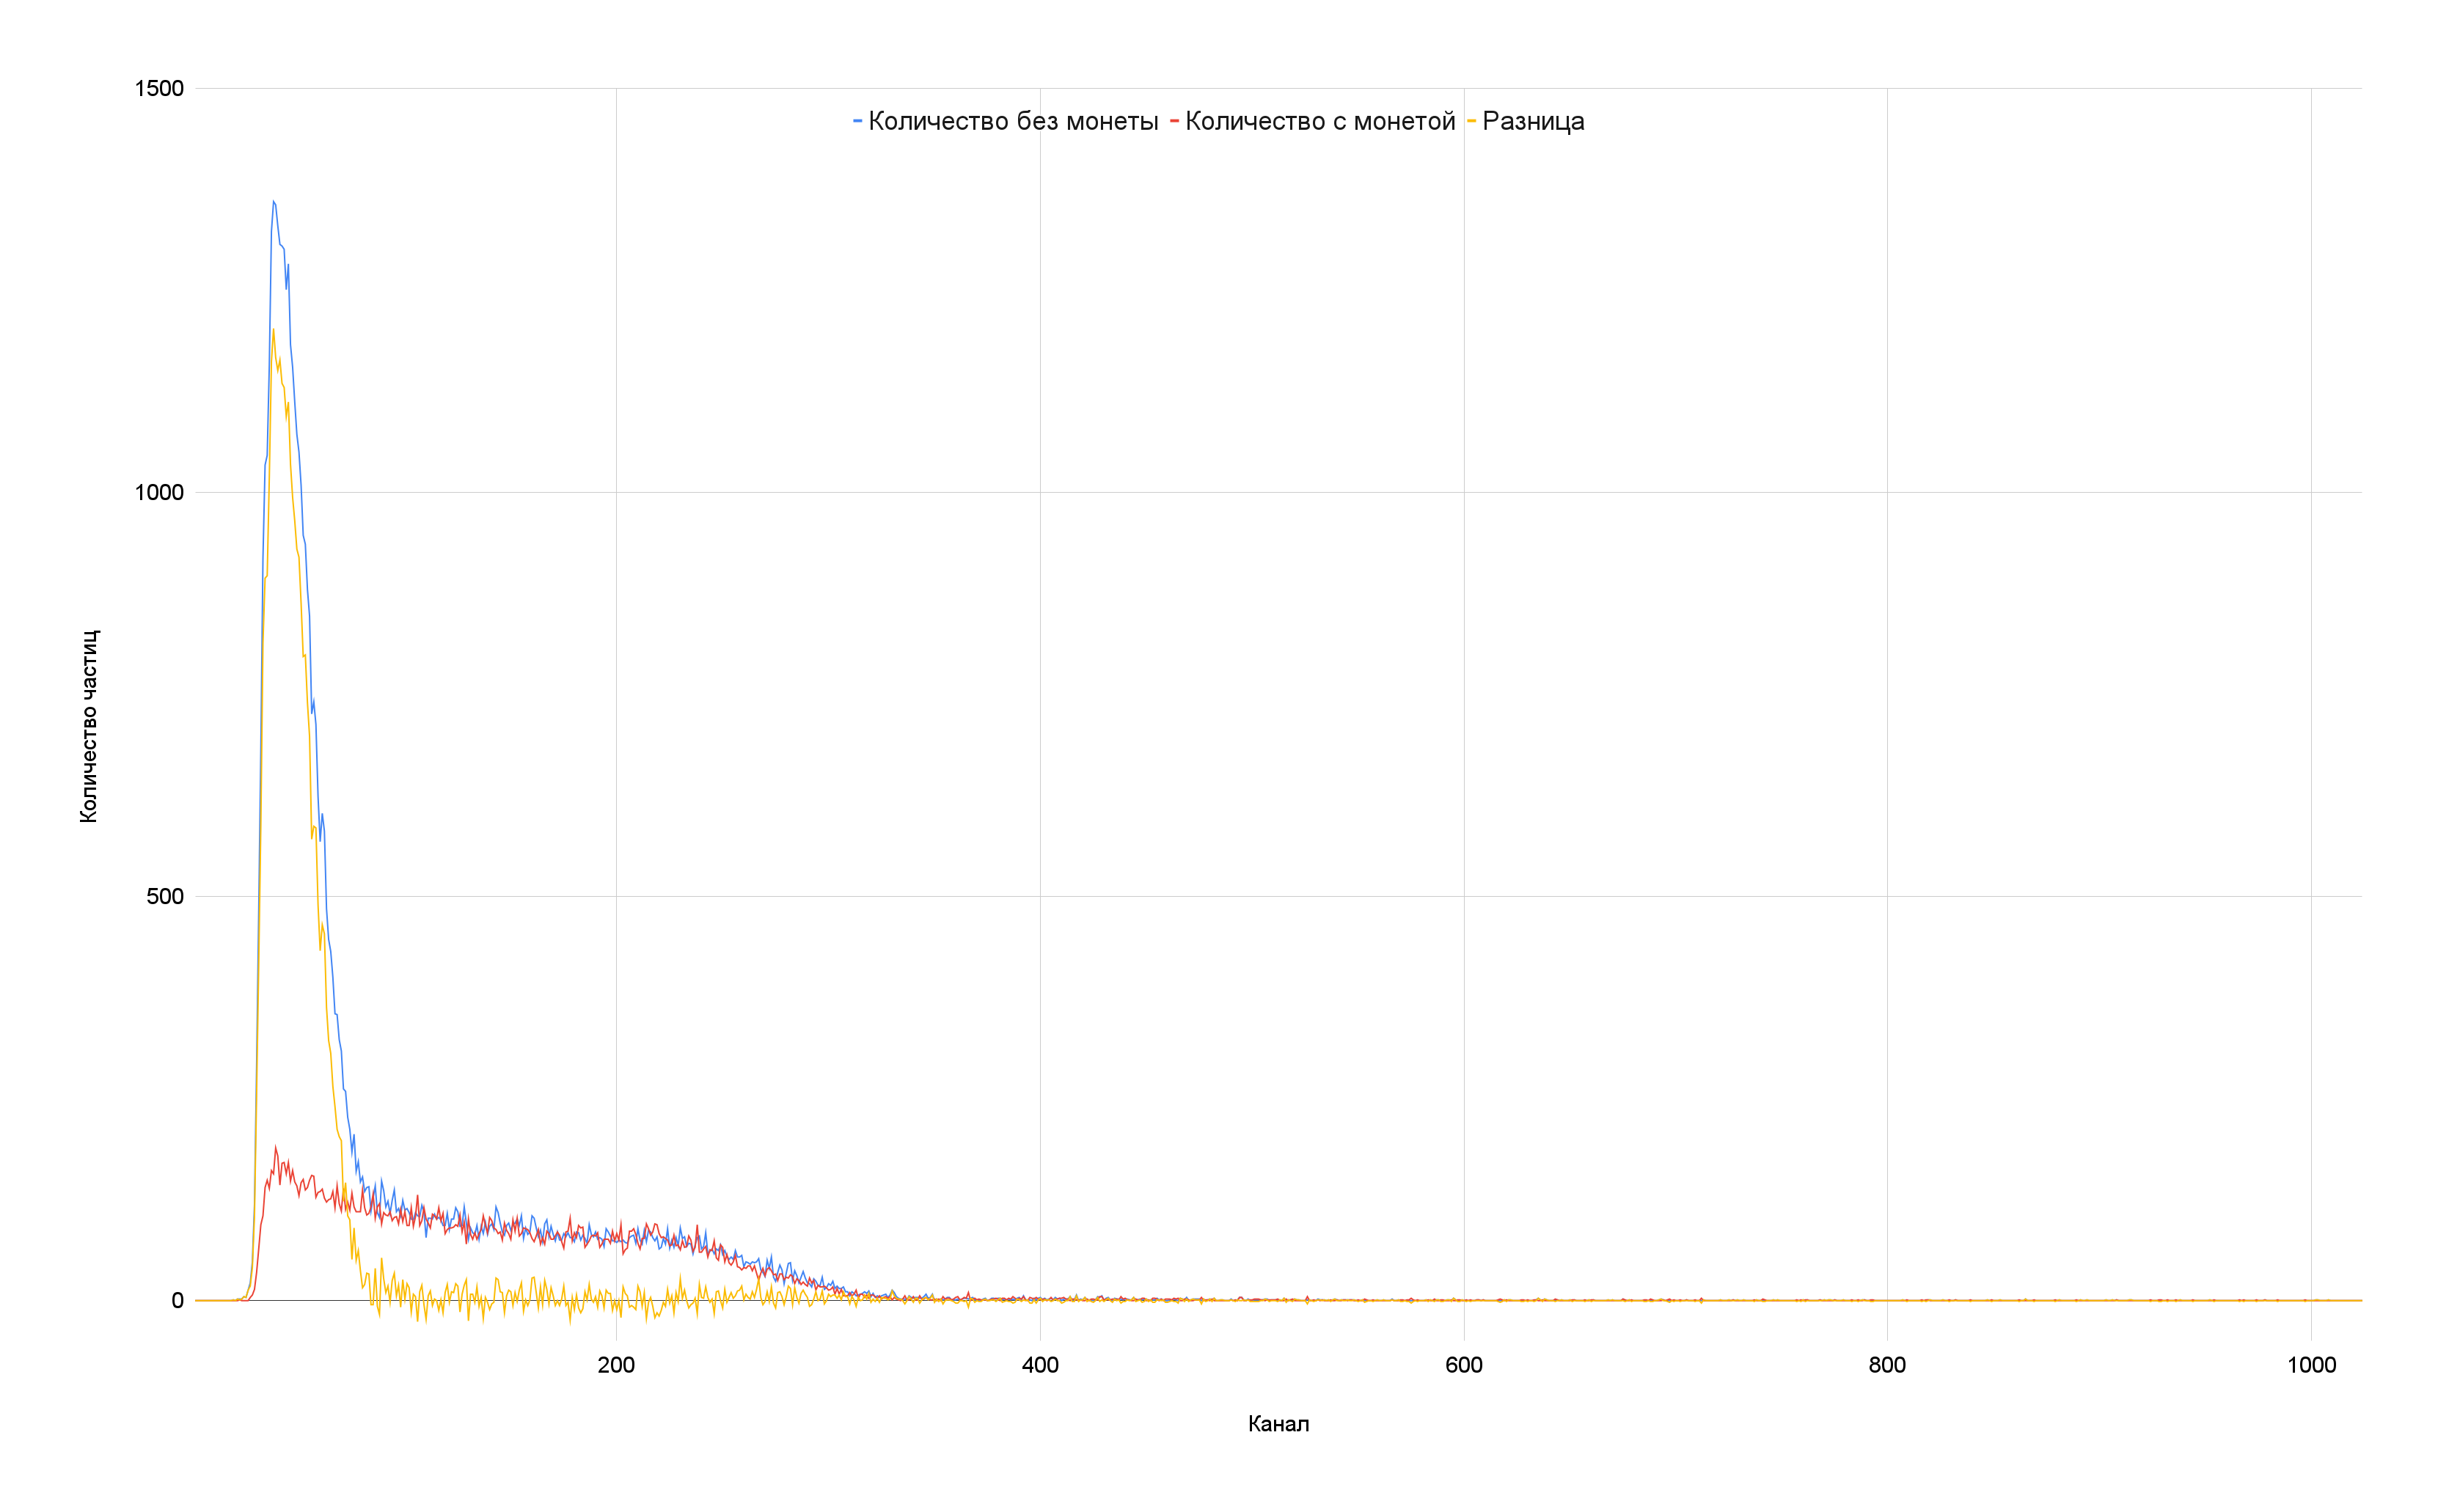
\includegraphics[width=\linewidth]{cobalt.png}}
        Рис 4. Спектры для кобальта без монеты и с монетой, разница спектров
      \end{minipage}
      \label{chart:cobalt}
    \end{figure}

    Граничная энергия электронов:$E_1 = 87/255 \approx 0.341$МэВ;
    $E_2 = 340/255 \approx 1.333$МэВ.

    Энергия края комптоновского рассеяния $\gamma$-квантов:
    $E_k = 258/255 \approx 1.012$МэВ.

    Теоретические значения: $E_1 = 0.314$МэВ; $E_2 = 1.480$МэВ.


  \newpage
  \section{Обработка данных для $^{22}Na$}

    \begin{figure}[h!]
      \begin{minipage}[h]{\linewidth}
        \center{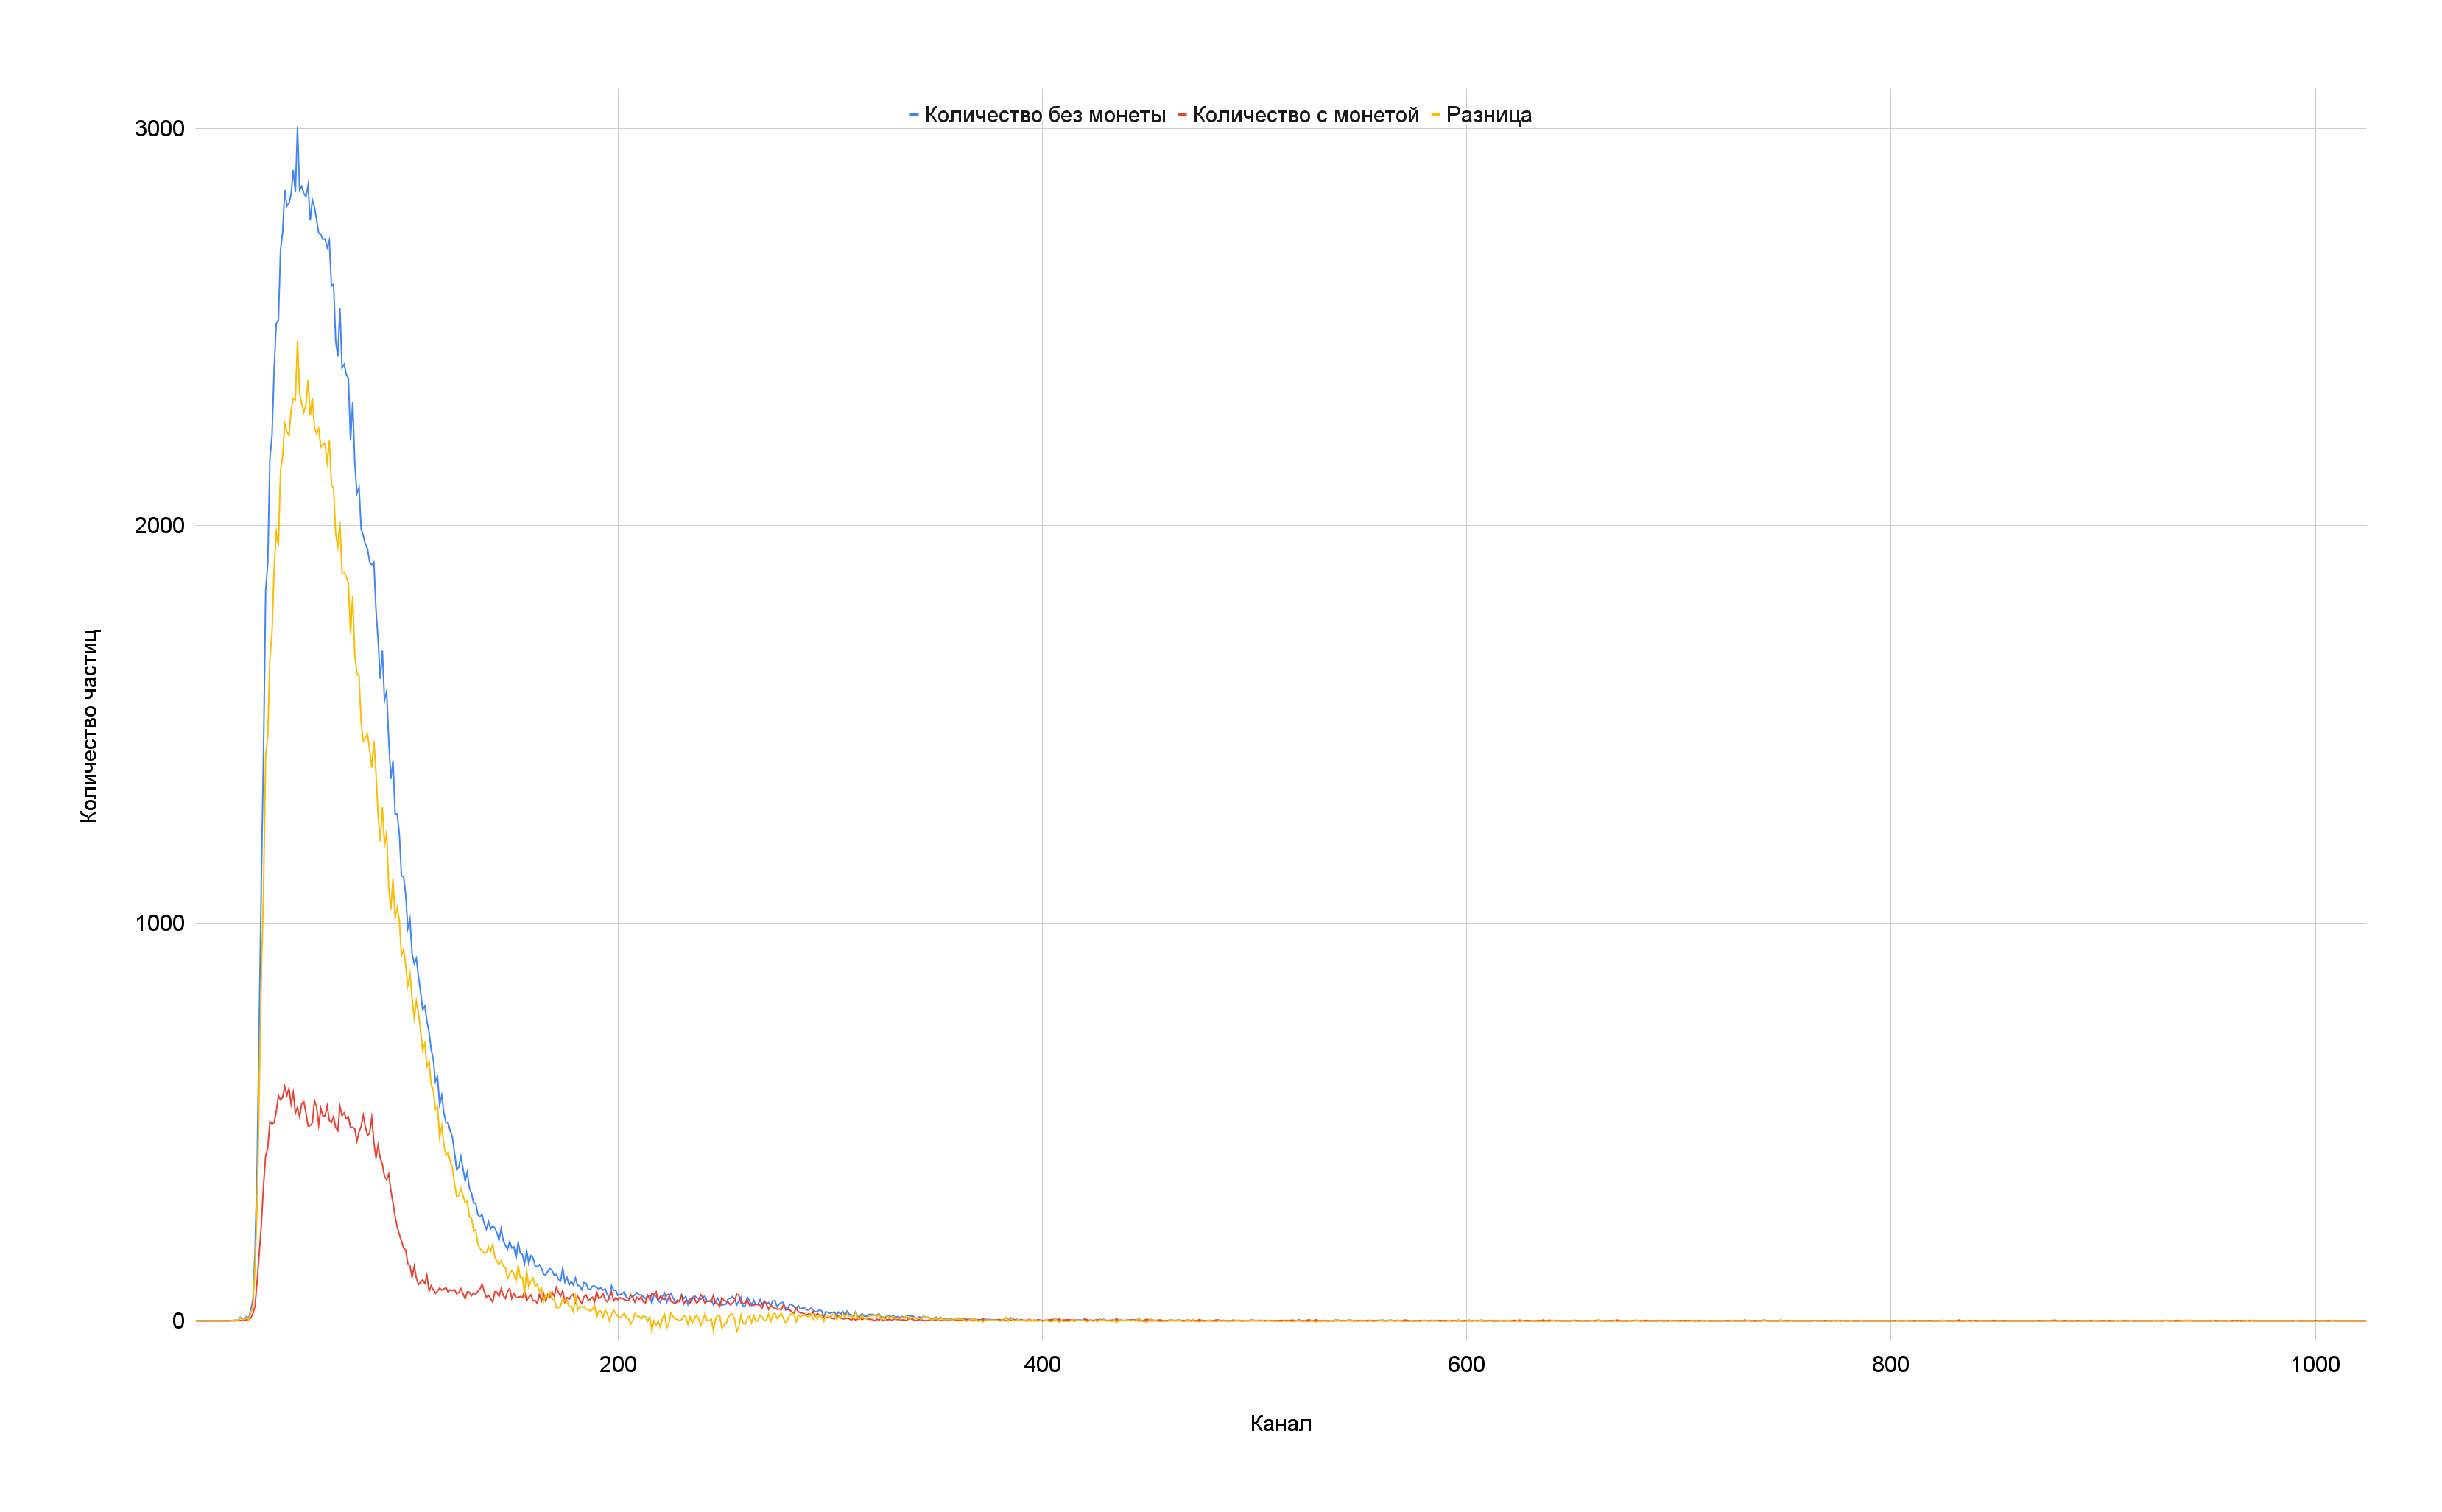
\includegraphics[width=\linewidth]{natrium.png}}
        Рис 5. Спектры для натрия без монеты и с монетой, разница спектров
      \end{minipage}
      \label{chart:natrium}
    \end{figure}

    Граничная энергия позитронов: $E_p = 193/255 \approx 0.757$МэВ.

    Энергии краев компотновсого рассеяния для $\gamma$-квантов:
    $E_1 = 84/255 \approx 0.329$МэВ; $E_2 = 257/255
    \approx 1.008$МэВ.

    Теоретические значения:$E_1 = 0.511$; $E_2 = 1.275$МэВ.


  \newpage
  \section{Вывод}

    В ходе выполнения работы мы получили следующие значения\\

    \begin{tabular}{ || c || c | c | c | c || }
      \hline
      Вещество & $E_{гр1}, МэВ$ & $E_{гр2}, МэВ$ & $E_{к1}, МэВ$ & $E_{к2},
      МэВ$ \\ \hline\hline
      Cs & $0,510$ & - & $0,413$ & - \\ \hline
      Sr & $0,569$ & $2,212$ & - & - \\ \hline
      Cl & $0,698$ & - & - & - \\ \hline
      Co & $0,341$ & $1,333$ & $1,012$ & - \\ \hline
      Na & $0,757$ & - & $0,329$ & $1,008$ \\
      \hline
    \end{tabular}\\

    Они в полной мере совпадают с теоретическими значениями этих величин.

\end{document}
